\documentclass[titlepage,a4paper]{article}

\usepackage{a4wide}
\usepackage[colorlinks=true,linkcolor=black,urlcolor=blue,bookmarksopen=true]{hyperref}
\usepackage{bookmark}
\usepackage{fancyhdr}
\usepackage[spanish]{babel}
\usepackage[utf8]{inputenc}
\usepackage[T1]{fontenc}
\usepackage{graphicx}
\usepackage{float}
\usepackage{listings}
\usepackage[table,xcdraw]{xcolor}
\usepackage{pdfpages}
\newcommand{\codigoMateria}{86.37 / 66.20}
\newcommand{\nombreMateria}{[86.37 / 66.20] Organización de Computadoras}
\newcommand{\curso}{2}
\usepackage{mips}
\usepackage{amssymb, amsmath, amsbsy} % librerias ams
\usepackage{cprotect}

\newcommand{\numeroTP}{0}
\newcommand{\tituloTP}{Trabajo práctico 1}
\newcommand{\descripcionTP}{Conjunto de instrucciones MIPS}

\newcommand{\facultad}{Facultad de Ingeniería}
\newcommand{\universidad}{Universidad de Buenos Aires}
\newcommand{\cuatrimestre}{2do Cuatrimestre de 2020}


\pagestyle{fancy} % Encabezado y pie de página
\fancyhf{}
\fancyhead[L]{TP1 - Conjunto de instrucciones MIPS}
\fancyhead[R]{Organización de Computadoras - FIUBA}
\renewcommand{\headrulewidth}{0.4pt}
\fancyfoot[C]{\thepage}
\renewcommand{\footrulewidth}{0.4pt}

\newcommand{\teammember}[3]{
	 #1 & #2 & \texttt{#3}\\
}

\begin{document}
\begin{titlepage} % Carátula
    \centering
      
\includegraphics[scale = 0.75]{images/logo_fiuba.png}\\[1.0 cm]	% Logo universidad
      \textsc{\LARGE \universidad}\\[0.5 cm]	% Nombre universidad
      \textsc{\Large \facultad}\\[0.5 cm]	% Facultad
      \textsc{\large \cuatrimestre}\\[1.0 cm]	% Cuatrimestre
    \centering
    
     \textsc{\Large \nombreMateria}\\[0.5 cm] % Nombre materia
      \textsc{\large Curso \curso}\\[0.4 cm]	% Curso
      
      \rule{\linewidth}{0.2 mm} \\[0.4 cm]
      { \huge \tituloTP}\\[0.5 cm]
      { \huge \bfseries}
      { \huge \bfseries \descripcionTP}\\
      \rule{\linewidth}{0.2 mm} \\[1 cm]
      
      
     \resizebox{12cm}{!}{
        \begin{tabular}{ | l | l | l | }
          \hline
          Padrón & Alumno & Email \\
          \hline
          \teammember{103442}{Lovera, Daniel}{dlovera@fi.uba.ar}
          \teammember{102914}{More, Agustín}{amore@fi.uba.ar}
          \teammember{99846}{Torresetti, Lisandro}{ltorresetti@fi.uba.ar}
          \hline
      	\end{tabular}
  	}
  	\vskip2cm
  	\Large Repositorio: \url{https://github.com/DanieLovera/Orga}
  	
\end{titlepage}


\tableofcontents % Índice general
\newpage

\lstdefinestyle{customC}{
  language=C,                % choose the language of the code
  backgroundcolor=\color[HTML]{fcfbfc},
  numbers=left,                   % where to put the line-numbers
  stepnumber=1,                   % the step between two line-numbers.        
  numbersep=10pt,                  % how far the line-numbers are from the code
  frame=l,	                   % adds a frame around the code
  showspaces=false,               % show spaces adding particular underscores
  showstringspaces=false,         % underline spaces within strings
  keywordstyle=\color[HTML]{6684e1},
  stringstyle=\color[HTML]{1fad83},     % string literal style
  commentstyle=\color[HTML]{999580},
  showtabs=false,                 % show tabs within strings adding particular underscores
  tabsize=2,                      % sets default tabsize to 2 spaces
  captionpos=b,                   % sets the caption-position to bottom
  breaklines=true,                % sets automatic line breaking
  breakatwhitespace=true,         % sets if automatic breaks should only happen at whitespace
  title=\lstname,                 % show the filename of files included with \lstinputlisting;
  postbreak=\mbox{\textcolor{darkgray}{$\hookrightarrow$}\space},
}

\section{Objetivos}\label{sec:objetivos}
Familiarizarse con el conjunto de instrucciones MIPS32 y el concepto de \verb|ABI|, realizando un programa que calcula el mínimo común múltiplo (\verb|mcm|) y el máximo común divisor (\verb|mcd|) entre dos números, utilizando para éste último el \textit{algoritmo de Euclides} \cite{euclidean_algorithm}.

\section{Introducción}\label{sec:intro}
El algoritmo de Euclides es un método antiguo y eficiente para calcular el máximo común divisor (\verb|mcd|) que se basa en lo siguiente: \newline

Al dividir \textit{a} entre \textit{b} (números enteros), se obtiene un cociente \textit{q} y un residuo \textit{r}. Es posible demostrar que el máximo común divisor de \textit{a} y \textit{b} es el mismo que el de \textit{b} y \textit{r}. Sea c el máximo común divisor de \textit{a} y \textit{b}, como $a = b * q + r$ y \textit{c} divide a \textit{a} y a \textit{b} divide también a \textit{r}. Si existiera otro número mayor que \textit{c} que divide a \textit{b} y a \textit{r}, también dividiría a \textit{a} , por lo que \textit{c} no sería el \verb|mcd| de \textit{a} y \textit{b} (lo que contradice la hipótesis). Este es el fundamento principal del algoritmo. \newline

Para hallar el \verb|mcm| entre dos números se utiliza el \verb|mcd|, dado que el \verb|mcm| entre dos números es el producto de ambos divido entre su \verb|mcd|.

$$mcm(a,b) = \frac{a * b}{mcd(a,b)}$$


%\section{Programa a implementar}\label{sec:programa_a_implementar}
%Utilizando el lenguaje `C' se implementa un codificador y %decodificador de texto en base64. La entrada será un archivo %especificado en el comando o el \textit{stdin} si ninguno es %especificado, y la salida será otro archivo también especificado en %el comando o el \textit{stdout} si ninguno es especificado.

\section{Detalles de implementación}\label{sec:detalles_implementacion}
El programa principal consta de dos rutinas externas importantes escritas en lenguaje \textit{assembly} para procesadores mips32, se encuentran programadas en los módulos \verb|mcd_euclides.S| y \verb|mcm_euclides.S|, las cuales se hicieron siguiendo una implementación realizada para soporte en \verb|C| (\verb|euclides_algorithm.c|) y siguen línea a línea este archivo de código fuente, además tienen asociados cada instrucción de alto nivel en \verb|C| a las instrucciones de bajo nivel en \textit{assembly}. A continuación se detallan cada una de ellas.


\cprotect\subsection{Módulo \verb|mcd_euclides.S|}
La subrutina contenida dentro de este módulo (\verb|mcd_euclides(unsigned int a, insigned int b)|), recibe dos parámetros y a su vez utiliza una variable local, por lo cual siguiendo la convención de la \verb|ABI| para mips32 se reservan 40 bytes de memoria en el stack, y en general se distribuye como se muestra a continuación.

\begin{figure}[H]
\centering
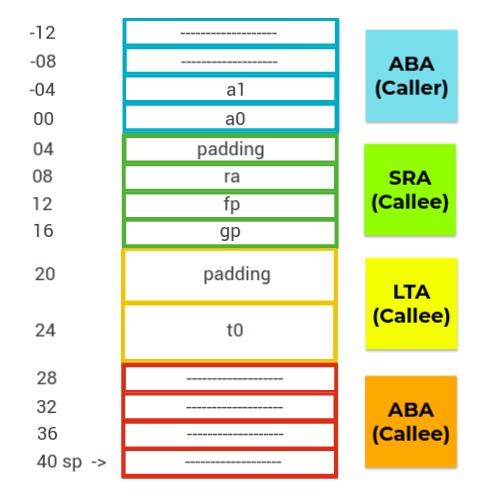
\includegraphics[width=0.4\textwidth]{images/stackMcdCall.jpeg}
\cprotect\caption{\label{fig:seq01}Stack general de subrutina \verb|mcd_euclides(unsigned int a, insigned int b)|}
\end{figure}

En la Figura \ref{fig:seq01} se incluye la sección \verb|ABA| (caller), la cual no pertenece a la función en cuestión, sin embargo, para mas claridad se incluyó debido a que por convención es el invocado es el que debe almacenar los parámetros recibidos en los registros dentro del stack del invocador. La primera función que llamará a \verb|mcd_euclides.S| es \verb|main.c| y se programo en alto nivel, por la tanto se confía en que esta función cumple con la convención necesaria. \\


El \verb|SRA| (callee) corresponde a los registros que el invocado debe respaldar por convención,  se incluye el registro \verb|ra| (junto al \verb|fp| y \verb|gp|) en esta región ya que esta es una función no hoja, y se debe evitar que las direcciones de retorno se sobrescriban en cada llamado a una nueva función. Observar que pese a que solo se necesitan 4 bytes (excluyendo los 8 bytes del registro \verb|fp| y \verb|gp|) para el registro \verb|ra|, se reservaron 8 bytes de stack extra para mantener la convención de alineación, por lo cual los 4 bytes restantes quedan rellenos con padding.\\

El \verb|LTA| (callee) no es necesario crearlo por convención, sin embargo para evitar trabajar únicamente con registros, lo cual haría el código mas complicado de entender y propenso a errores, se decidió crearla para priorizar la claridad del código y facilitar el trabajo de programación. Nuevamente se reservan 4 bytes adicionales por cuestiones de alineación.\\
	
Finalmente la complejidad de esta implementación reside en el llamado recursivo que realiza. Esta es la razón por la cual estamos obligados a reservar 16 bytes extras que corresponden a la sección \verb|ABA| (callee), como se mencionó, por convención se debe reservar espacio en memoria para que la función invocada pueda almacenar sus parámetros en esta sección, una vez se realice el nuevo llamado, la función pasara de su condición de invocada a invocadora una y otra vez hasta que finalice su condición de corte y empiece a retornar el resultado por cada uno de los nuevos marcos de pila que se crearon hasta la primera función invocadora (el \verb|main|). Se debe señalar que por seguir la convención de la \verb|ABI| inicialmente, los llamados recursivos resultaron ser algo trivial pues la función ya sabe que debe guardar sus parámetros en la función invocadora y cuánto espacio tiene que reservar, por lo cual no fallará cuando tenga que llamarse a si misma.\\

A continuación se muestra como se ve el stack de la función invocada una vez finaliza sus tareas y esta lista para retornar o invocarse nuevamente.\\

\begin{figure}[H]
\centering
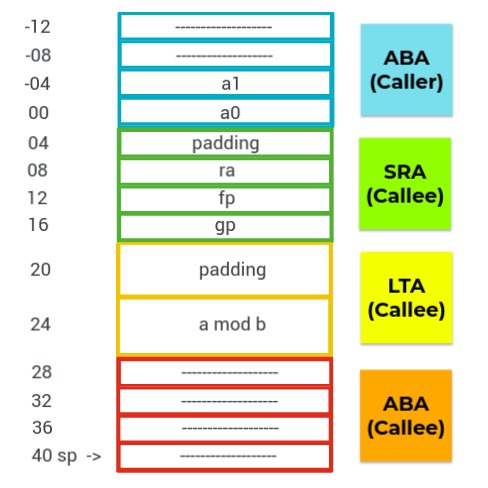
\includegraphics[width=0.4\textwidth]{images/stackMcdEjec.jpeg}
\cprotect\caption{\label{fig:seq02}Stack en ejecución de la subrutina \verb|mcd_euclides(unsigned int a, insigned int b)|}
\end{figure}
	
Se observa que todas las posiciones del stack se mantienen sin cambios con respecto a la anterior versión con excepción del registro \verb|t0| esto se debe a que fue el que se utilizó para guardar el contenido de la variable local de la rutina, los demás registros están forzados a ser almacenados como respaldo por convención.\\

El código escrito para este módulo puede encontrarse en la sección apéndice \ref{apendice:codigo_assembly} código MIPS32 \verb|mcd_euclides|.

\cprotect\subsection{Módulo \verb|mcm_euclides.S|}
La subrutina contenida dentro de este módulo (\verb|mcm_euclides(unsigned int a, insigned int b)|), recibe dos parámetros y a su vez utiliza dos variables locales, por lo cual siguiendo la convención de la \verb|ABI| para mips32 se reservan 40 bytes de memoria en el stack, y en general se distribuye como se muestra en la figura \ref{fig:seq03}.\\

\begin{figure}[H]
\centering
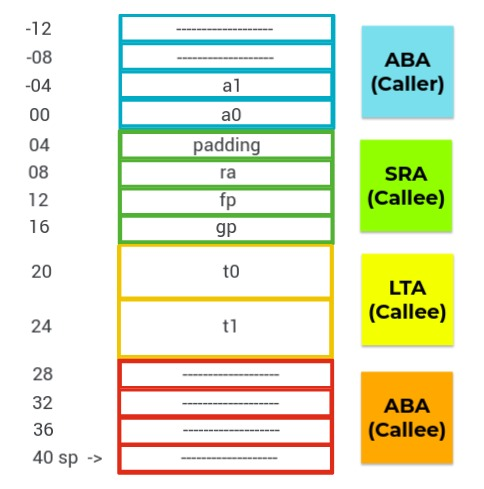
\includegraphics[width=0.4\textwidth]{images/stackMcmCall.jpeg}
\cprotect\caption{\label{fig:seq03}Stack general de la subrutina \verb|mcm_euclides(unsigned int a, unsigned int b)|}
\end{figure}

Para esta rutina se observa que la estructura general del stack es muy parecida a la anterior, esto se debe a que son programas cortos y muy parecidos entre sí, de hecho el funcionamiento de esta rutina depende de \verb|mcd_euclides(unsigned int a, insigned int b)| y vista en alto nivel únicamente requiere dos operaciones aritméticas sencillas para obtener el resultado esperado. 

Como se mencionó anteriormente la sección \verb|ABA| (caller) no pertenece a la función en cuestión, sin embargo, para mantener coherencia con las imágenes que están siendo presentadas se incluyó de nuevo. Igualmente esta función confía en que el programa principal escrito en C respete la convención establecida al momento de invocarla.\\ 

Las sección \verb|LRA| se repite debido a que es obligatoria tenerla y al ser una función no hoja se deben reservar 16 bytes con 4 de padding para esta sección y además los correspondientes 16 bytes extras reservados del \verb|ABA| para la función invocada.\\

En esta oportunidad la función de alto nivel en C requiere dos variables locales y pese a que el código assembly era igualmente sencillo, se decidió seguir con esta idea de ser cuidadosos a la hora de programar en lugar de buscar eficiencia, por lo cual el \verb|LTA| no requiere ningún tipo de padding. En ejecución únicamente se modificara esta sección y pasara a tomar los siguientes valores:

\begin{figure}[H]
\centering
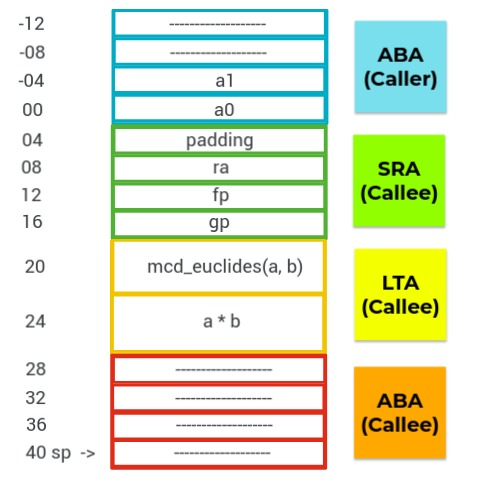
\includegraphics[width=0.4\textwidth]{images/stackMcmEjec.jpeg}
\cprotect\caption{\label{fig:seq04}Stack general de la subrutina \verb|mcm_euclides(unsigned int a, unsigned int b)|}
\end{figure}

Esta función tiene el inconveniente de que trabaja con enteros sin signos de 32 bits e involucra una multiplicación entre ambos, por lo tanto se corre el riesgo de obtener resultados inesperados si la multiplicación entre a y b es mayor a $2^3^2$, ya que no podrá ser representado correctamente.

\section{Compilación y ejecución}

\subsection{Compilación}
Para compilar el programa implementado se incluyo un archivo \verb|Makefile|   en el repositorio, se debe ejecutar el comando \verb|make| \cite{makefile}, esto generará los siguientes archivos: 

\begin{itemize}
    \item \verb|mcm_euclides.o|: Código objeto del programa que contiene el programa para calcular el mínimo común múltiplo.
    \item \verb|mcd_euclides.o|: Código objeto del programa que contiene el programa para calcular el máximo común múltiplo.
    \item \verb|main.o|: Código objeto del programa principal.
    \item \verb|common|: Código ejecutable.
\end{itemize}
En caso que se requiera limpiar automáticamente el \verb|build| realizado se puede ejecutar el comando \verb|make clean|, y removerá todos los archivos generados por el comando \verb|make|.

\subsection{Ejecución}
Para ejecutar el archivo compilado:
\begin{verbatim}
    ./common [Opciones] PARÁMETRO1 PARÁMETRO2
\end{verbatim}

\subsubsection{Descripción de parámetros}
\begin{itemize}
    \cprotect\item[\verb|-V|] {-}{-}version: Muestra la versión y sale del programa.
    \cprotect\item[\verb|-h|] {-}{-}help: Muestra información de ayuda de cómo ejecutar el programa y sale del programa.
    \cprotect\item[\verb|-o|] {-}{-}output: Path para el archivo de salida (en caso de indicar el carácter `\verb|-|' o no se utiliza el parámetro, se utilizará el \verb|stdout|).
    \cprotect\item[\verb|-d|] {-}{-}divisor: Calcula únicamente el máximo común divisor.
    \cprotect\item[\verb|-m|] {-}{-}multiple: Calcula únicamente el mínimo común múltiplo.
\end{itemize}

\subsubsection{Ejemplos de ejecución}

Calcular el mínimo común múltiplo o máximo común divisor de dos números, por ejemplo 256 y 192, y mostrarlo en pantalla, se puede realizar de cualquiera de las siguientes maneras:

\begin{verbatim}
    ./common -d -o - 256 192
\end{verbatim}

\begin{verbatim}
    ./common -m -o - 256 192
\end{verbatim}

\begin{verbatim}
    ./common -m 256 192
\end{verbatim}

\begin{verbatim}
    ./common -d 256 192
\end{verbatim}

Si deseamos calcular el \verb|mcm| y \verb|mcd| a la vez, y mostrarlo en la pantalla, se puede realizar de las siguientes maneras:

\begin{verbatim}
    ./common -o - 256 192
\end{verbatim}

\begin{verbatim}
    ./common 256 192
\end{verbatim}

\subsubsection{Pruebas automatizadas}

Ejecutar el comando \verb|make testing| para correr automáticamente todas las pruebas.

\section{Pruebas}
\lstdefinestyle{test_run_style}{
    breaklines=true,
    breakatwhitespace=false,
    postbreak=\mbox{\textcolor{darkgray}{$\hookrightarrow$}\space},
    frame=single,
    framesep=10pt
}

\subsection{Prueba 1}

Se prueba que al indicar un número negativo, se lo toma como un número fuera de rango (y no como un parámetro) en el caso de restringir por la opción \verb|divisor| de la forma larga.

\begin{lstlisting}[style=test_run_style]
./common --divisor 10 -10

Error: Número fuera de rango [2, 2147483647).

\end{lstlisting}

\subsection{Prueba 2}

Se prueba la opción de indicar el output como \verb|stdout| pero sin indicar los números, con lo cual se espera un mensaje de error indicando el problema.
\begin{lstlisting}[style=test_run_style]
./common -o -

Error: Faltan los números.

\end{lstlisting}

\subsection{Prueba 3}

Se prueba indicando explícitamente ambas opciones de \verb|divisor| y \verb|multiple| y se obtiene el resultado esperado. 
\begin{lstlisting}[style=test_run_style]
./common -d -m 10 20
10
20

\end{lstlisting}

\subsection{Prueba 4}

Se prueba indicando explícitamente la opción \verb|divisor| de forma corta y se obtiene el resultado esperado en el \verb|stdout|.

\begin{lstlisting}[style=test_run_style]
./common -o - -d 10 20
10
\end{lstlisting}

\subsection{Prueba 5}

Se prueba la opción \verb|version| de la forma corta.
\begin{lstlisting}[style=test_run_style]
./common -V
Version 1.0
\end{lstlisting}

\subsection{Prueba 6}

Se prueba la opción más básica que reconoce el sistema con un número fuera de rango por exceso. Se espera que se obtenga mensaje indicando que algún número se encuentra fuera de rango.

\begin{lstlisting}[style=test_run_style]
./common 10 10000000000000000000000

Error: Número fuera de rango [2, 2147483647).

\end{lstlisting}

\subsection{Prueba 7}

Se prueba la opción más básica que reconoce el sistema con ambos números dentro del rango, pero en los extremos. Se espera obtener los valores correspondiente sin ningún error. 
\begin{lstlisting}[style=test_run_style]
./common 2 2147483646
2
2147483646

\end{lstlisting}

\subsection{Prueba 8}

Se prueba valores fuera de rango por rango inferior. Se espera obtener mensaje de error `Fuera de rango'
\begin{lstlisting}[style=test_run_style]
./common 1 1

Error: Número fuera de rango [2, 2147483647).

\end{lstlisting}

\subsection{Prueba 9}

Se prueba el valor que se encuantra al principio del intervalo admitido, se espera obtener el resultado sin ningún mensaje de error. En particular, al tratarse de $f(2, 2)$ se espera obtener $mcm(2, 2) = 2$ y $mcd(2, 2) = 2$
\begin{lstlisting}[style=test_run_style]
./common 2 2
2
2
\end{lstlisting}


\subsection{Prueba 10}
Se prueba ambos valores fuera de rango, con parámetros adicioneles, se espera el mensaje indicando `Número fuera de rango'.
\begin{lstlisting}[style=test_run_style]
./common -o - -10 1

Error: Número fuera de rango [2, 2147483647).

\end{lstlisting}

\subsection{Prueba 11}

Se prueba la opción más básica que reconoce el sistema con ambos números dentro del rango, pero en los extremos invertidos. Se espera obtener los valores correspondiente sin ningún error. 
\begin{lstlisting}[style=test_run_style]
./common 2147483646 2
2
2147483646
\end{lstlisting}


\subsection{Prueba 12}


Se prueba indicando explícitamente la opción \verb|multiple| de forma corta.
\begin{lstlisting}[style=test_run_style]
./common -m 10 20
20
\end{lstlisting}

\subsection{Prueba 13}

Se prueban ambas opciones, esta vez con el \verb|output| al \verb|stdout| explícito con el carácter `\verb|-|'
\begin{lstlisting}[style=test_run_style]
./common -o - 10 20
10
20
\end{lstlisting}

\subsection{Prueba 14}
Se prueba la función \verb|divisor| de forma larga con números medianos.
\begin{lstlisting}[style=test_run_style]
./common --divisor 192 168
24
\end{lstlisting}

\subsection{Prueba 15}
Se prueba con entrada dos números iguales no primos.
\begin{lstlisting}[style=test_run_style]
./common 10 10
10
10


\end{lstlisting}

\subsection{Prueba 16}
Se prueba el programa con las opciones básicas, con un sólo parámetro numérico, se espera un mensaje de error.
\begin{lstlisting}[style=test_run_style]
./common 10

Error: Faltan los números.
\end{lstlisting}

\subsection{Prueba 17}
Se prueba el programa con las opciones básicas, con ningún parámetro numérico, se espera un mensaje de error.
\begin{lstlisting}[style=test_run_style]
./common 

Error: Faltan los números.

\end{lstlisting}
\subsection{Prueba 18}

Se prueba el programa con las opciones básicas, con un número negativo, se espera un mensaje de error de número fuera de rango.
\begin{lstlisting}[style=test_run_style]
./common -10 5

Error: Número fuera de rango [2, 2147483647).
\end{lstlisting}

\subsection{Prueba 19}
Se prueban dos números iguales y primos.
\begin{lstlisting}[style=test_run_style]
./common 11 11
11
11

\end{lstlisting}
\subsection{Prueba 20}
Se prueba la opción de \verb|help| en la versión corta.
\begin{lstlisting}[style=test_run_style]
./common -h
Usage:
	common -h
	common -V
	common [options] M N
Options:
	-h, --help Prints usage information.
	-V, --version Prints version information.
	-o, --output Path to output file.
	-d --divisor Just the divisor
	-m --multiple Just the multiple


\end{lstlisting}
\subsection{Prueba 21}
Se prueba la opción \verb|version| de la forma corta, con parámetros adicionales, se espera que el sistema solo tome en consideración la primer acción y que ignore los demás parámetros. 
\begin{lstlisting}[style=test_run_style]
./common -V 10 10
Version 1.0

\end{lstlisting}

\section{Conclusiones}
El objetivo principal del trabajo consistió en el entendimiento de la ABI de mips32, a partir de los módulos implementados en este lenguaje, esta convención es útil para evitar errores entre librerías escritas por distintos programadores y se comprobó que se cumple debido a que las partes escritas en C que fueron ensambladas por el compilador no tuvieron problemas con las escritas por nosotros, por ejemplo la función main reservó espacio automáticamente en el stack para las funciones .S por lo cual no se corrompió la memoria de esta. \newline
Por otra parte, al escribir las funciones de mcm y mcd de 'backup' en C, se pudo ver la diferencia y la complejidad en escribir el mismo programa a más bajo nivel que C, como es el caso de mips32. Los programas realizan lo mismo de una manera similar, pero al ser de tan bajo nivel mips32, escribir el código de las funciones lo volvió mucho más lento.


\newpage
\appendix
\section{Código}
\subsection{Código en C}
\label{apendice:codigo_c}
\subsubsection{main.c}
\begin{lstlisting}[style=customC]
#include <stdio.h>
#include <stdlib.h>
#include <limits.h>
#include <stdbool.h>
#include <getopt.h>
#include <string.h>
#include <ctype.h>

#define MAX_FUNCTIONS_TO_RUN 2
#define STDIN_PARAM_IDENTIFIER "-"
#define INVALID_RESULT 0
#define MIN_VALUE_INPUT 2
#define MAX_VALUE_INPUT INT_MAX
#define CORRECT_INPUT 0
#define ALPHA_ERROR 1
#define NEGATIVE_ERROR 2

extern unsigned int mcd_euclides(unsigned int a, unsigned int b);
extern unsigned int mcm_euclides(unsigned int a, unsigned int b);

typedef unsigned int (*bin_operation_t) (unsigned int, unsigned int);

bool is_in_range(unsigned int value, unsigned int min, unsigned int max) {
	return min <= value && value < max;
}

int is_a_number(char* num){
	if (num[0] != '-' && !isdigit(num[0])) return ALPHA_ERROR;

	if (num[0] == '-' || isdigit(num[0])){
		for (size_t i = 1; i < strlen(num); i++){
			if (!isdigit(num[i])) return ALPHA_ERROR;
		}
		if (num[0] == '-') return NEGATIVE_ERROR;

		return CORRECT_INPUT;
	}

	return ALPHA_ERROR;
}

bool correct_input(char* num1, char* num2){
	int result_1 = is_a_number(num1);
	int result_2 = is_a_number(num2);
	if (result_1 + result_2 == CORRECT_INPUT) return true;

	if (result_1 == ALPHA_ERROR || result_2 == ALPHA_ERROR){
		fprintf(stderr, "Error: deben ingresarse numeros no cadenas de texto\n");
		return false;
	}

	fprintf(stderr, "Error: Los numeros ingresados deben ser positivos y estar en el rango [%d, %d]\n", MIN_VALUE_INPUT,
		MAX_VALUE_INPUT);

}

unsigned int bin_operation_decorator(bin_operation_t operation, unsigned int a, 
									 unsigned int b) {
	if (!is_in_range(a, MIN_VALUE_INPUT, MAX_VALUE_INPUT) || 
		!is_in_range(b, MIN_VALUE_INPUT, MAX_VALUE_INPUT))
		return INVALID_RESULT;
	return operation(a, b);
}

void show_usage() {
	printf("Usage:\n"
		   "	common -h\n"
		   "	common -V\n"
		   "	common [options] M N\n"
		   "Options:\n"
		   "	-h, --help Prints usage information.\n"
		   "	-V, --version Prints version information.\n"
		   "	-o, --output Path to output file.\n"
		   "	-d --divisor Just the divisor\n"
		   "	-m --multiple Just the multiple\n");
}

void show_version() {
	printf("Version 1.0\n");
}

int parse_argv(int argc, char *argv[], FILE* output_file, 
			   bin_operation_t functions[], int *functions_to_run) {
	opterr = 0; // getopt suprime los mensajes de error
	static struct option argument_options[] = {
		{"help", no_argument, 0, 'h'},
		{"version", no_argument, 0, 'V'},
		{"output", required_argument, 0, 'o'},
		{"divisor", no_argument, 0, 'd'},
		{"multiple", no_argument, 0, 'm'},
		{0, 0, 0, 0} // Lo pide getopt
	};

	int opt;
	int option_index = 0;
	while ((opt = getopt_long(argc, argv, "hVo:dm", argument_options, 
														&option_index)) != -1) {
		switch (opt) {
		case 'h':
			show_usage();
			exit(EXIT_SUCCESS);
		case 'V':
			show_version();
			exit(EXIT_SUCCESS);
		case 'o':
			if (strcmp(optarg, STDIN_PARAM_IDENTIFIER) != 0) {
				output_file = fopen(optarg, "w");
				if (!output_file) {
					fprintf(stderr, "No se pudo abrir el archivo %s\n", optarg);
					exit(EXIT_FAILURE);
				}
			}
			break;
		case 'd':
			functions[(*functions_to_run)++] = mcd_euclides;
			break;
		case 'm':
			functions[(*functions_to_run)++] = mcm_euclides;
			break;
		case 0:
			printf("long option %s", argument_options[option_index].name);
			if (optarg) 
				printf(" with arg %s", optarg);
			printf("\n");
			break;
		case '?':
			// TODO: Hacer un tratado mejor de errores
			show_usage();
			exit(EXIT_FAILURE);
		default:
			show_usage();
			exit(EXIT_FAILURE);
		}
		option_index = 0;
	}
	return optind;
}


int main(int argc, char *argv[]) {
	FILE* output_file = stdout;
	bin_operation_t functions[] = {
		mcd_euclides,
		mcm_euclides
	};
	int functions_to_run = 0;
	
	int last_index = parse_argv(argc, argv, output_file, functions, 
								&functions_to_run);

	if (!output_file) {
		fprintf(stderr, "No se pudo acceder al archivo de salida.\n");
		exit(EXIT_FAILURE);
	}
	
	if (!argv[last_index] || !argv[last_index + 1]) {
		fprintf(stderr, "Faltan los números.\n");
		show_usage();
		exit(EXIT_FAILURE);
	}

	if(!correct_input(argv[last_index], argv[last_index + 1])) exit(EXIT_FAILURE);

	unsigned int a = atoi(argv[last_index]);
	unsigned int b = atoi(argv[last_index + 1]);

	if (functions_to_run == 0)
		functions_to_run = MAX_FUNCTIONS_TO_RUN;

	for (int i = 0; i < functions_to_run; i++) {
		unsigned int result = bin_operation_decorator(functions[i], a, b);
		if (result == INVALID_RESULT) {
			fprintf(stderr, "Número fuera de rango [%d, %d).\n", 
											MIN_VALUE_INPUT, MAX_VALUE_INPUT);
			break;
		}
		fprintf(output_file, "%u\n", result);
	}

	if (output_file != stdout)
		fclose(output_file);

	return EXIT_SUCCESS;
}
\end{lstlisting}

\subsection{Código MIPS32}
\label{apendice:codigo_assembly}
\subsubsection{mcd euclides.S}
\begin{lstlisting}[style=customC]
#include <sys/regdef.h>

.text
.align 2
.globl mcd_euclides
.ent mcd_euclides 
/*
 * Espacio reservado para el stack de la funcion
 */
#define STACK_SIZE 40

/*
 * Argument building area (ABA) caller
 * 16 bytes
 * - a1
 * - a0
 */
#define O_A1 STACK_SIZE + 4 
#define O_A0 STACK_SIZE

/* 
 * Save register area (SRA) callee
 * 16 bytes
 * - padding
 * - ra
 * - fp
 * - gp
 */
#define O_RA STACK_SIZE - 8
#define O_FP STACK_SIZE - 12 
#define O_GP STACK_SIZE - 16

/*
 * Local and temporary area (LTA) callee
 * 8 bytes
 * - padding
 * - t0
 */
#define O_L0 STACK_SIZE - 24

/*
 * Argument building area (ABA) callee
 * 16 bytes
 * Se reserva para el llamado recursivo
 */

/* Firma de la funcion:
 * unsigned int mcd_euclides(unsigned int a, unsigned int b);
 */
mcd_euclides:
	.frame fp, STACK_SIZE, ra	
	addiu sp, sp, -STACK_SIZE
	sw ra, O_RA(sp)
	sw fp, O_FP(sp)
	.cprestore O_GP
	move fp, sp
	sw a0, O_A0(fp)
	sw a1, O_A1(fp)
	
	/* unsigned int r = 0 */
	move t0, zero
	sw t0, O_L0(fp)
	
	/* if (b == 0) */
	lw t0, O_A1(fp)
	beqz t0, return
	
	/* r = (a % b); */
	lw t0, O_A0(fp)
	lw t1, O_A1(fp)
	divu t0, t0, t1
	mfhi t0
	sw t0, O_L0(fp)	

return_recursivo:
	/* return mcd_euclides(b, r); */
	lw a0, O_A1(fp)
	lw a1, O_L0(fp)
	jal mcd_euclides
	
	lw ra, O_RA(sp)
	lw fp, O_FP(sp)
	lw gp, O_GP(sp)	
	addiu sp, sp, STACK_SIZE
	jr ra	

return:
	/* return a; */
	lw v0, O_A0(sp)

	lw ra, O_RA(sp)
	lw fp, O_FP(sp)
	lw gp, O_GP(sp)	
	addiu sp, sp, STACK_SIZE
	jr ra
.end mcd_euclides
\end{lstlisting}

\subsubsection{mcm euclides.S}
\begin{lstlisting}[style=customC]
#include <sys/regdef.h>

.text
.align 2
.globl mcm_euclides
.extern mcd_euclides
.ent mcm_euclides 
/*
 * Espacio reservado para el stack de la funcion
 */
#define STACK_SIZE 40

/*
 * Argument building area (ABA) caller
 * 16 bytes
 * - a1
 * - a0
 */
#define O_A1 STACK_SIZE + 4 
#define O_A0 STACK_SIZE

/* 
 * Save register area (SRA) callee
 * 16 bytes
 * - padding
 * - ra
 * - fp
 * - gp
 */
#define O_RA STACK_SIZE - 8
#define O_FP STACK_SIZE - 12 
#define O_GP STACK_SIZE - 16

/*
 * Local and temporary area (LTA) callee
 * 8 bytes
 * - t0
 * - t1
 */
#define O_L0 STACK_SIZE - 20
#define O_L1 STACK_SIZE - 24

/*
 * Argument building area (ABA) callee
 * 16 bytes
 * Se reserva para el llamado a mcd_euclides
 */

/* Firma de la funcion:
 * unsigned int mcm_euclides(unsigned int a, unsigned int b);
 */
mcm_euclides:
	.frame fp, STACK_SIZE, ra	
	addiu sp, sp, -STACK_SIZE
	sw ra, O_RA(sp)
	sw fp, O_FP(sp)
	.cprestore O_GP
	move fp, sp
	sw a0, O_A0(fp)
	sw a1, O_A1(fp)
	
	/* unsigned int mcd = mcd_euclides(a, b); */
	lw a0, O_A0(fp)
	lw a1, O_A1(fp)
	jal mcd_euclides
	sw v0, O_L0(sp)

	/* unsigned int a_x_b = (a * b); */
	lw t0, O_A0(fp)
	lw t1, O_A1(fp)
	multu t0, t1
	mflo t0
	sw t0, O_L1(fp)

return:
	/* return (a_x_b / mcd); */
	lw t0, O_L0(fp)
	lw t1, O_L1(fp)
	divu v0, t1, t0

	lw ra, O_RA(sp)
	lw fp, O_FP(sp)
	lw gp, O_GP(sp)	
	addiu sp, sp, STACK_SIZE
	jr ra
.end mcm_euclides
\end{lstlisting}

\subsubsection{main.s}
\begin{lstlisting}[style=customC]
	.file	1 "main.c"
	.section .mdebug.abi32
	.previous
	.nan	legacy
	.module	fp=xx
	.module	nooddspreg
	.abicalls
	.text
	.align	2
	.globl	is_in_range
	.set	nomips16
	.set	nomicromips
	.ent	is_in_range
	.type	is_in_range, @function
is_in_range:
	.frame	$fp,8,$31		# vars= 0, regs= 1/0, args= 0, gp= 0
	.mask	0x40000000,-4
	.fmask	0x00000000,0
	.set	noreorder
	.set	nomacro
	addiu	$sp,$sp,-8
	sw	$fp,4($sp)
	move	$fp,$sp
	sw	$4,8($fp)
	sw	$5,12($fp)
	sw	$6,16($fp)
	lw	$3,12($fp)
	lw	$2,8($fp)
	sltu	$2,$2,$3
	bne	$2,$0,$L2
	nop

	lw	$3,8($fp)
	lw	$2,16($fp)
	sltu	$2,$3,$2
	beq	$2,$0,$L2
	nop

	li	$2,1			# 0x1
	b	$L3
	nop

$L2:
	move	$2,$0
$L3:
	andi	$2,$2,0x1
	andi	$2,$2,0x00ff
	move	$sp,$fp
	lw	$fp,4($sp)
	addiu	$sp,$sp,8
	jr	$31
	nop

	.set	macro
	.set	reorder
	.end	is_in_range
	.size	is_in_range, .-is_in_range
	.align	2
	.globl	is_a_number
	.set	nomips16
	.set	nomicromips
	.ent	is_a_number
	.type	is_a_number, @function
is_a_number:
	.frame	$fp,40,$31		# vars= 8, regs= 2/0, args= 16, gp= 8
	.mask	0xc0000000,-4
	.fmask	0x00000000,0
	.set	noreorder
	.cpload	$25
	.set	nomacro
	addiu	$sp,$sp,-40
	sw	$31,36($sp)
	sw	$fp,32($sp)
	move	$fp,$sp
	.cprestore	16
	sw	$4,40($fp)
	lw	$2,40($fp)
	lb	$3,0($2)
	li	$2,45			# 0x2d
	beq	$3,$2,$L6
	nop

	lw	$2,%call16(__ctype_b_loc)($28)
	move	$25,$2
	.reloc	1f,R_MIPS_JALR,__ctype_b_loc
1:	jalr	$25
	nop

	lw	$28,16($fp)
	lw	$3,0($2)
	lw	$2,40($fp)
	lb	$2,0($2)
	sll	$2,$2,1
	addu	$2,$3,$2
	lhu	$2,0($2)
	andi	$2,$2,0x8
	bne	$2,$0,$L6
	nop

	li	$2,1			# 0x1
	b	$L7
	nop

$L6:
	lw	$2,40($fp)
	lb	$3,0($2)
	li	$2,45			# 0x2d
	beq	$3,$2,$L8
	nop

	lw	$2,%call16(__ctype_b_loc)($28)
	move	$25,$2
	.reloc	1f,R_MIPS_JALR,__ctype_b_loc
1:	jalr	$25
	nop

	lw	$28,16($fp)
	lw	$3,0($2)
	lw	$2,40($fp)
	lb	$2,0($2)
	sll	$2,$2,1
	addu	$2,$3,$2
	lhu	$2,0($2)
	andi	$2,$2,0x8
	beq	$2,$0,$L9
	nop

$L8:
	li	$2,1			# 0x1
	sw	$2,24($fp)
	b	$L10
	nop

$L12:
	lw	$2,%call16(__ctype_b_loc)($28)
	move	$25,$2
	.reloc	1f,R_MIPS_JALR,__ctype_b_loc
1:	jalr	$25
	nop

	lw	$28,16($fp)
	lw	$3,0($2)
	lw	$4,40($fp)
	lw	$2,24($fp)
	addu	$2,$4,$2
	lb	$2,0($2)
	sll	$2,$2,1
	addu	$2,$3,$2
	lhu	$2,0($2)
	andi	$2,$2,0x8
	bne	$2,$0,$L11
	nop

	li	$2,1			# 0x1
	b	$L7
	nop

$L11:
	lw	$2,24($fp)
	addiu	$2,$2,1
	sw	$2,24($fp)
$L10:
	lw	$4,40($fp)
	lw	$2,%call16(strlen)($28)
	move	$25,$2
	.reloc	1f,R_MIPS_JALR,strlen
1:	jalr	$25
	nop

	lw	$28,16($fp)
	move	$3,$2
	lw	$2,24($fp)
	sltu	$2,$2,$3
	bne	$2,$0,$L12
	nop

	lw	$2,40($fp)
	lb	$3,0($2)
	li	$2,45			# 0x2d
	bne	$3,$2,$L13
	nop

	li	$2,2			# 0x2
	b	$L7
	nop

$L13:
	move	$2,$0
	b	$L7
	nop

$L9:
	li	$2,1			# 0x1
$L7:
	move	$sp,$fp
	lw	$31,36($sp)
	lw	$fp,32($sp)
	addiu	$sp,$sp,40
	jr	$31
	nop

	.set	macro
	.set	reorder
	.end	is_a_number
	.size	is_a_number, .-is_a_number
	.rdata
	.align	2
$LC0:
	.ascii	"Error: deben ingresarse numeros no cadenas de texto\012\000"
	.align	2
$LC1:
	.ascii	"Error: Los numeros ingresados deben ser positivos y esta"
	.ascii	"r en el rango [%d, %d]\012\000"
	.text
	.align	2
	.globl	correct_input
	.set	nomips16
	.set	nomicromips
	.ent	correct_input
	.type	correct_input, @function
correct_input:
	.frame	$fp,40,$31		# vars= 8, regs= 2/0, args= 16, gp= 8
	.mask	0xc0000000,-4
	.fmask	0x00000000,0
	.set	noreorder
	.cpload	$25
	.set	nomacro
	addiu	$sp,$sp,-40
	sw	$31,36($sp)
	sw	$fp,32($sp)
	move	$fp,$sp
	.cprestore	16
	sw	$4,40($fp)
	sw	$5,44($fp)
	lw	$4,40($fp)
	lw	$2,%got(is_a_number)($28)
	move	$25,$2
	.reloc	1f,R_MIPS_JALR,is_a_number
1:	jalr	$25
	nop

	lw	$28,16($fp)
	sw	$2,24($fp)
	lw	$4,44($fp)
	lw	$2,%got(is_a_number)($28)
	move	$25,$2
	.reloc	1f,R_MIPS_JALR,is_a_number
1:	jalr	$25
	nop

	lw	$28,16($fp)
	sw	$2,28($fp)
	lw	$3,24($fp)
	lw	$2,28($fp)
	addu	$2,$3,$2
	bne	$2,$0,$L15
	nop

	li	$2,1			# 0x1
	b	$L16
	nop

$L15:
	lw	$3,24($fp)
	li	$2,1			# 0x1
	beq	$3,$2,$L17
	nop

	lw	$3,28($fp)
	li	$2,1			# 0x1
	bne	$3,$2,$L18
	nop

$L17:
	lw	$2,%got(stderr)($28)
	lw	$2,0($2)
	move	$7,$2
	li	$6,52			# 0x34
	li	$5,1			# 0x1
	lw	$2,%got($LC0)($28)
	addiu	$4,$2,%lo($LC0)
	lw	$2,%call16(fwrite)($28)
	move	$25,$2
	.reloc	1f,R_MIPS_JALR,fwrite
1:	jalr	$25
	nop

	lw	$28,16($fp)
	move	$2,$0
	b	$L16
	nop

$L18:
	lw	$2,%got(stderr)($28)
	lw	$3,0($2)
	li	$2,2147418112			# 0x7fff0000
	ori	$7,$2,0xffff
	li	$6,2			# 0x2
	lw	$2,%got($LC1)($28)
	addiu	$5,$2,%lo($LC1)
	move	$4,$3
	lw	$2,%call16(fprintf)($28)
	move	$25,$2
	.reloc	1f,R_MIPS_JALR,fprintf
1:	jalr	$25
	nop

	lw	$28,16($fp)
	b	$L14
	nop

$L16:
$L14:
	move	$sp,$fp
	lw	$31,36($sp)
	lw	$fp,32($sp)
	addiu	$sp,$sp,40
	jr	$31
	nop

	.set	macro
	.set	reorder
	.end	correct_input
	.size	correct_input, .-correct_input
	.align	2
	.globl	bin_operation_decorator
	.set	nomips16
	.set	nomicromips
	.ent	bin_operation_decorator
	.type	bin_operation_decorator, @function
bin_operation_decorator:
	.frame	$fp,32,$31		# vars= 0, regs= 2/0, args= 16, gp= 8
	.mask	0xc0000000,-4
	.fmask	0x00000000,0
	.set	noreorder
	.cpload	$25
	.set	nomacro
	addiu	$sp,$sp,-32
	sw	$31,28($sp)
	sw	$fp,24($sp)
	move	$fp,$sp
	.cprestore	16
	sw	$4,32($fp)
	sw	$5,36($fp)
	sw	$6,40($fp)
	li	$2,2147418112			# 0x7fff0000
	ori	$6,$2,0xffff
	li	$5,2			# 0x2
	lw	$4,36($fp)
	lw	$2,%got(is_in_range)($28)
	move	$25,$2
	.reloc	1f,R_MIPS_JALR,is_in_range
1:	jalr	$25
	nop

	lw	$28,16($fp)
	xori	$2,$2,0x1
	andi	$2,$2,0x00ff
	bne	$2,$0,$L20
	nop

	li	$2,2147418112			# 0x7fff0000
	ori	$6,$2,0xffff
	li	$5,2			# 0x2
	lw	$4,40($fp)
	lw	$2,%got(is_in_range)($28)
	move	$25,$2
	.reloc	1f,R_MIPS_JALR,is_in_range
1:	jalr	$25
	nop

	lw	$28,16($fp)
	xori	$2,$2,0x1
	andi	$2,$2,0x00ff
	beq	$2,$0,$L21
	nop

$L20:
	move	$2,$0
	b	$L22
	nop

$L21:
	lw	$2,32($fp)
	lw	$5,40($fp)
	lw	$4,36($fp)
	move	$25,$2
	jalr	$25
	nop

	lw	$28,16($fp)
$L22:
	move	$sp,$fp
	lw	$31,28($sp)
	lw	$fp,24($sp)
	addiu	$sp,$sp,32
	jr	$31
	nop

	.set	macro
	.set	reorder
	.end	bin_operation_decorator
	.size	bin_operation_decorator, .-bin_operation_decorator
	.rdata
	.align	2
$LC2:
	.ascii	"Usage:\012\011common -h\012\011common -V\012\011common ["
	.ascii	"options] M N\012Options:\012\011-h, --help Prints usage "
	.ascii	"information.\012\011-V, --version Prints version informa"
	.ascii	"tion.\012\011-o, --output Path to output file.\012\011-d"
	.ascii	" --divisor Just the divisor\012\011-m --multiple Just th"
	.ascii	"e multiple\000"
	.text
	.align	2
	.globl	show_usage
	.set	nomips16
	.set	nomicromips
	.ent	show_usage
	.type	show_usage, @function
show_usage:
	.frame	$fp,32,$31		# vars= 0, regs= 2/0, args= 16, gp= 8
	.mask	0xc0000000,-4
	.fmask	0x00000000,0
	.set	noreorder
	.cpload	$25
	.set	nomacro
	addiu	$sp,$sp,-32
	sw	$31,28($sp)
	sw	$fp,24($sp)
	move	$fp,$sp
	.cprestore	16
	lw	$2,%got($LC2)($28)
	addiu	$4,$2,%lo($LC2)
	lw	$2,%call16(puts)($28)
	move	$25,$2
	.reloc	1f,R_MIPS_JALR,puts
1:	jalr	$25
	nop

	lw	$28,16($fp)
	nop
	move	$sp,$fp
	lw	$31,28($sp)
	lw	$fp,24($sp)
	addiu	$sp,$sp,32
	jr	$31
	nop

	.set	macro
	.set	reorder
	.end	show_usage
	.size	show_usage, .-show_usage
	.rdata
	.align	2
$LC3:
	.ascii	"Version 1.0\000"
	.text
	.align	2
	.globl	show_version
	.set	nomips16
	.set	nomicromips
	.ent	show_version
	.type	show_version, @function
show_version:
	.frame	$fp,32,$31		# vars= 0, regs= 2/0, args= 16, gp= 8
	.mask	0xc0000000,-4
	.fmask	0x00000000,0
	.set	noreorder
	.cpload	$25
	.set	nomacro
	addiu	$sp,$sp,-32
	sw	$31,28($sp)
	sw	$fp,24($sp)
	move	$fp,$sp
	.cprestore	16
	lw	$2,%got($LC3)($28)
	addiu	$4,$2,%lo($LC3)
	lw	$2,%call16(puts)($28)
	move	$25,$2
	.reloc	1f,R_MIPS_JALR,puts
1:	jalr	$25
	nop

	lw	$28,16($fp)
	nop
	move	$sp,$fp
	lw	$31,28($sp)
	lw	$fp,24($sp)
	addiu	$sp,$sp,32
	jr	$31
	nop

	.set	macro
	.set	reorder
	.end	show_version
	.size	show_version, .-show_version
	.rdata
	.align	2
$LC4:
	.ascii	"-\000"
	.align	2
$LC5:
	.ascii	"w\000"
	.align	2
$LC6:
	.ascii	"No se pudo abrir el archivo %s\012\000"
	.align	2
$LC7:
	.ascii	"long option %s\000"
	.align	2
$LC8:
	.ascii	" with arg %s\000"
	.align	2
$LC9:
	.ascii	"hVo:dm\000"
	.text
	.align	2
	.globl	parse_argv
	.set	nomips16
	.set	nomicromips
	.ent	parse_argv
	.type	parse_argv, @function
parse_argv:
	.frame	$fp,48,$31		# vars= 8, regs= 2/0, args= 24, gp= 8
	.mask	0xc0000000,-4
	.fmask	0x00000000,0
	.set	noreorder
	.cpload	$25
	.set	nomacro
	addiu	$sp,$sp,-48
	sw	$31,44($sp)
	sw	$fp,40($sp)
	move	$fp,$sp
	.cprestore	24
	sw	$4,48($fp)
	sw	$5,52($fp)
	sw	$6,56($fp)
	sw	$7,60($fp)
	lw	$2,%got(opterr)($28)
	sw	$0,0($2)
	sw	$0,36($fp)
	b	$L26
	nop

$L39:
	lw	$2,32($fp)
	li	$3,100			# 0x64
	beq	$2,$3,$L28
	nop

	slt	$3,$2,101
	beq	$3,$0,$L29
	nop

	li	$3,63			# 0x3f
	beq	$2,$3,$L30
	nop

	li	$3,86			# 0x56
	beq	$2,$3,$L31
	nop

	beq	$2,$0,$L32
	nop

	b	$L27
	nop

$L29:
	li	$3,109			# 0x6d
	beq	$2,$3,$L33
	nop

	li	$3,111			# 0x6f
	beq	$2,$3,$L34
	nop

	li	$3,104			# 0x68
	bne	$2,$3,$L27
	nop

	lw	$2,%got(show_usage)($28)
	move	$25,$2
	.reloc	1f,R_MIPS_JALR,show_usage
1:	jalr	$25
	nop

	lw	$28,24($fp)
	move	$4,$0
	lw	$2,%call16(exit)($28)
	move	$25,$2
	.reloc	1f,R_MIPS_JALR,exit
1:	jalr	$25
	nop

$L31:
	lw	$2,%got(show_version)($28)
	move	$25,$2
	.reloc	1f,R_MIPS_JALR,show_version
1:	jalr	$25
	nop

	lw	$28,24($fp)
	move	$4,$0
	lw	$2,%call16(exit)($28)
	move	$25,$2
	.reloc	1f,R_MIPS_JALR,exit
1:	jalr	$25
	nop

$L34:
	lw	$2,%got(optarg)($28)
	lw	$3,0($2)
	lw	$2,%got($LC4)($28)
	addiu	$5,$2,%lo($LC4)
	move	$4,$3
	lw	$2,%call16(strcmp)($28)
	move	$25,$2
	.reloc	1f,R_MIPS_JALR,strcmp
1:	jalr	$25
	nop

	lw	$28,24($fp)
	beq	$2,$0,$L41
	nop

	lw	$2,%got(optarg)($28)
	lw	$3,0($2)
	lw	$2,%got($LC5)($28)
	addiu	$5,$2,%lo($LC5)
	move	$4,$3
	lw	$2,%call16(fopen)($28)
	move	$25,$2
	.reloc	1f,R_MIPS_JALR,fopen
1:	jalr	$25
	nop

	lw	$28,24($fp)
	sw	$2,56($fp)
	lw	$2,56($fp)
	bne	$2,$0,$L41
	nop

	lw	$2,%got(stderr)($28)
	lw	$3,0($2)
	lw	$2,%got(optarg)($28)
	lw	$2,0($2)
	move	$6,$2
	lw	$2,%got($LC6)($28)
	addiu	$5,$2,%lo($LC6)
	move	$4,$3
	lw	$2,%call16(fprintf)($28)
	move	$25,$2
	.reloc	1f,R_MIPS_JALR,fprintf
1:	jalr	$25
	nop

	lw	$28,24($fp)
	li	$4,1			# 0x1
	lw	$2,%call16(exit)($28)
	move	$25,$2
	.reloc	1f,R_MIPS_JALR,exit
1:	jalr	$25
	nop

$L28:
	lw	$2,64($fp)
	lw	$2,0($2)
	addiu	$4,$2,1
	lw	$3,64($fp)
	sw	$4,0($3)
	sll	$2,$2,2
	lw	$3,60($fp)
	addu	$2,$3,$2
	lw	$3,%got(mcd_euclides)($28)
	sw	$3,0($2)
	b	$L37
	nop

$L33:
	lw	$2,64($fp)
	lw	$2,0($2)
	addiu	$4,$2,1
	lw	$3,64($fp)
	sw	$4,0($3)
	sll	$2,$2,2
	lw	$3,60($fp)
	addu	$2,$3,$2
	lw	$3,%got(mcm_euclides)($28)
	sw	$3,0($2)
	b	$L37
	nop

$L32:
	lw	$3,36($fp)
	lw	$2,%got(argument_options.2692)($28)
	sll	$3,$3,4
	addiu	$2,$2,%lo(argument_options.2692)
	addu	$2,$3,$2
	lw	$2,0($2)
	move	$5,$2
	lw	$2,%got($LC7)($28)
	addiu	$4,$2,%lo($LC7)
	lw	$2,%call16(printf)($28)
	move	$25,$2
	.reloc	1f,R_MIPS_JALR,printf
1:	jalr	$25
	nop

	lw	$28,24($fp)
	lw	$2,%got(optarg)($28)
	lw	$2,0($2)
	beq	$2,$0,$L38
	nop

	lw	$2,%got(optarg)($28)
	lw	$2,0($2)
	move	$5,$2
	lw	$2,%got($LC8)($28)
	addiu	$4,$2,%lo($LC8)
	lw	$2,%call16(printf)($28)
	move	$25,$2
	.reloc	1f,R_MIPS_JALR,printf
1:	jalr	$25
	nop

	lw	$28,24($fp)
$L38:
	li	$4,10			# 0xa
	lw	$2,%call16(putchar)($28)
	move	$25,$2
	.reloc	1f,R_MIPS_JALR,putchar
1:	jalr	$25
	nop

	lw	$28,24($fp)
	b	$L37
	nop

$L30:
	lw	$2,%got(show_usage)($28)
	move	$25,$2
	.reloc	1f,R_MIPS_JALR,show_usage
1:	jalr	$25
	nop

	lw	$28,24($fp)
	li	$4,1			# 0x1
	lw	$2,%call16(exit)($28)
	move	$25,$2
	.reloc	1f,R_MIPS_JALR,exit
1:	jalr	$25
	nop

$L27:
	lw	$2,%got(show_usage)($28)
	move	$25,$2
	.reloc	1f,R_MIPS_JALR,show_usage
1:	jalr	$25
	nop

	lw	$28,24($fp)
	li	$4,1			# 0x1
	lw	$2,%call16(exit)($28)
	move	$25,$2
	.reloc	1f,R_MIPS_JALR,exit
1:	jalr	$25
	nop

$L41:
	nop
$L37:
	sw	$0,36($fp)
$L26:
	addiu	$2,$fp,36
	sw	$2,16($sp)
	lw	$2,%got(argument_options.2692)($28)
	addiu	$7,$2,%lo(argument_options.2692)
	lw	$2,%got($LC9)($28)
	addiu	$6,$2,%lo($LC9)
	lw	$5,52($fp)
	lw	$4,48($fp)
	lw	$2,%call16(getopt_long)($28)
	move	$25,$2
	.reloc	1f,R_MIPS_JALR,getopt_long
1:	jalr	$25
	nop

	lw	$28,24($fp)
	sw	$2,32($fp)
	lw	$3,32($fp)
	li	$2,-1			# 0xffffffffffffffff
	bne	$3,$2,$L39
	nop

	lw	$2,%got(optind)($28)
	lw	$2,0($2)
	move	$sp,$fp
	lw	$31,44($sp)
	lw	$fp,40($sp)
	addiu	$sp,$sp,48
	jr	$31
	nop

	.set	macro
	.set	reorder
	.end	parse_argv
	.size	parse_argv, .-parse_argv
	.rdata
	.align	2
$LC10:
	.ascii	"No se pudo acceder al archivo de salida.\012\000"
	.align	2
$LC11:
	.ascii	"Faltan los n\303\272meros.\012\000"
	.align	2
$LC12:
	.ascii	"N\303\272mero fuera de rango [%d, %d).\012\000"
	.align	2
$LC13:
	.ascii	"%u\012\000"
	.text
	.align	2
	.globl	main
	.set	nomips16
	.set	nomicromips
	.ent	main
	.type	main, @function
main:
	.frame	$fp,80,$31		# vars= 40, regs= 2/0, args= 24, gp= 8
	.mask	0xc0000000,-4
	.fmask	0x00000000,0
	.set	noreorder
	.cpload	$25
	.set	nomacro
	addiu	$sp,$sp,-80
	sw	$31,76($sp)
	sw	$fp,72($sp)
	move	$fp,$sp
	.cprestore	24
	sw	$4,80($fp)
	sw	$5,84($fp)
	lw	$2,%got(stdout)($28)
	lw	$2,0($2)
	sw	$2,36($fp)
	lw	$2,%got(mcd_euclides)($28)
	sw	$2,56($fp)
	lw	$2,%got(mcm_euclides)($28)
	sw	$2,60($fp)
	sw	$0,64($fp)
	addiu	$3,$fp,56
	addiu	$2,$fp,64
	sw	$2,16($sp)
	move	$7,$3
	lw	$6,36($fp)
	lw	$5,84($fp)
	lw	$4,80($fp)
	lw	$2,%got(parse_argv)($28)
	move	$25,$2
	.reloc	1f,R_MIPS_JALR,parse_argv
1:	jalr	$25
	nop

	lw	$28,24($fp)
	sw	$2,40($fp)
	lw	$2,36($fp)
	bne	$2,$0,$L43
	nop

	lw	$2,%got(stderr)($28)
	lw	$2,0($2)
	move	$7,$2
	li	$6,41			# 0x29
	li	$5,1			# 0x1
	lw	$2,%got($LC10)($28)
	addiu	$4,$2,%lo($LC10)
	lw	$2,%call16(fwrite)($28)
	move	$25,$2
	.reloc	1f,R_MIPS_JALR,fwrite
1:	jalr	$25
	nop

	lw	$28,24($fp)
	li	$4,1			# 0x1
	lw	$2,%call16(exit)($28)
	move	$25,$2
	.reloc	1f,R_MIPS_JALR,exit
1:	jalr	$25
	nop

$L43:
	lw	$2,40($fp)
	sll	$2,$2,2
	lw	$3,84($fp)
	addu	$2,$3,$2
	lw	$2,0($2)
	beq	$2,$0,$L44
	nop

	lw	$2,40($fp)
	addiu	$2,$2,1
	sll	$2,$2,2
	lw	$3,84($fp)
	addu	$2,$3,$2
	lw	$2,0($2)
	bne	$2,$0,$L45
	nop

$L44:
	lw	$2,%got(stderr)($28)
	lw	$2,0($2)
	move	$7,$2
	li	$6,21			# 0x15
	li	$5,1			# 0x1
	lw	$2,%got($LC11)($28)
	addiu	$4,$2,%lo($LC11)
	lw	$2,%call16(fwrite)($28)
	move	$25,$2
	.reloc	1f,R_MIPS_JALR,fwrite
1:	jalr	$25
	nop

	lw	$28,24($fp)
	lw	$2,%got(show_usage)($28)
	move	$25,$2
	.reloc	1f,R_MIPS_JALR,show_usage
1:	jalr	$25
	nop

	lw	$28,24($fp)
	li	$4,1			# 0x1
	lw	$2,%call16(exit)($28)
	move	$25,$2
	.reloc	1f,R_MIPS_JALR,exit
1:	jalr	$25
	nop

$L45:
	lw	$2,40($fp)
	sll	$2,$2,2
	lw	$3,84($fp)
	addu	$2,$3,$2
	lw	$4,0($2)
	lw	$2,40($fp)
	addiu	$2,$2,1
	sll	$2,$2,2
	lw	$3,84($fp)
	addu	$2,$3,$2
	lw	$2,0($2)
	move	$5,$2
	lw	$2,%got(correct_input)($28)
	move	$25,$2
	.reloc	1f,R_MIPS_JALR,correct_input
1:	jalr	$25
	nop

	lw	$28,24($fp)
	xori	$2,$2,0x1
	andi	$2,$2,0x00ff
	beq	$2,$0,$L46
	nop

	li	$4,1			# 0x1
	lw	$2,%call16(exit)($28)
	move	$25,$2
	.reloc	1f,R_MIPS_JALR,exit
1:	jalr	$25
	nop

$L46:
	lw	$2,40($fp)
	sll	$2,$2,2
	lw	$3,84($fp)
	addu	$2,$3,$2
	lw	$2,0($2)
	move	$4,$2
	lw	$2,%call16(atoi)($28)
	move	$25,$2
	.reloc	1f,R_MIPS_JALR,atoi
1:	jalr	$25
	nop

	lw	$28,24($fp)
	sw	$2,44($fp)
	lw	$2,40($fp)
	addiu	$2,$2,1
	sll	$2,$2,2
	lw	$3,84($fp)
	addu	$2,$3,$2
	lw	$2,0($2)
	move	$4,$2
	lw	$2,%call16(atoi)($28)
	move	$25,$2
	.reloc	1f,R_MIPS_JALR,atoi
1:	jalr	$25
	nop

	lw	$28,24($fp)
	sw	$2,48($fp)
	lw	$2,64($fp)
	bne	$2,$0,$L47
	nop

	li	$2,2			# 0x2
	sw	$2,64($fp)
$L47:
	sw	$0,32($fp)
	b	$L48
	nop

$L51:
	lw	$2,32($fp)
	sll	$2,$2,2
	addiu	$3,$fp,32
	addu	$2,$3,$2
	lw	$2,24($2)
	lw	$6,48($fp)
	lw	$5,44($fp)
	move	$4,$2
	lw	$2,%got(bin_operation_decorator)($28)
	move	$25,$2
	.reloc	1f,R_MIPS_JALR,bin_operation_decorator
1:	jalr	$25
	nop

	lw	$28,24($fp)
	sw	$2,52($fp)
	lw	$2,52($fp)
	bne	$2,$0,$L49
	nop

	lw	$2,%got(stderr)($28)
	lw	$3,0($2)
	li	$2,2147418112			# 0x7fff0000
	ori	$7,$2,0xffff
	li	$6,2			# 0x2
	lw	$2,%got($LC12)($28)
	addiu	$5,$2,%lo($LC12)
	move	$4,$3
	lw	$2,%call16(fprintf)($28)
	move	$25,$2
	.reloc	1f,R_MIPS_JALR,fprintf
1:	jalr	$25
	nop

	lw	$28,24($fp)
	b	$L50
	nop

$L49:
	lw	$6,52($fp)
	lw	$2,%got($LC13)($28)
	addiu	$5,$2,%lo($LC13)
	lw	$4,36($fp)
	lw	$2,%call16(fprintf)($28)
	move	$25,$2
	.reloc	1f,R_MIPS_JALR,fprintf
1:	jalr	$25
	nop

	lw	$28,24($fp)
	lw	$2,32($fp)
	addiu	$2,$2,1
	sw	$2,32($fp)
$L48:
	lw	$2,64($fp)
	lw	$3,32($fp)
	slt	$2,$3,$2
	bne	$2,$0,$L51
	nop

$L50:
	lw	$2,%got(stdout)($28)
	lw	$2,0($2)
	lw	$3,36($fp)
	beq	$3,$2,$L52
	nop

	lw	$4,36($fp)
	lw	$2,%call16(fclose)($28)
	move	$25,$2
	.reloc	1f,R_MIPS_JALR,fclose
1:	jalr	$25
	nop

	lw	$28,24($fp)
$L52:
	move	$2,$0
	move	$sp,$fp
	lw	$31,76($sp)
	lw	$fp,72($sp)
	addiu	$sp,$sp,80
	jr	$31
	nop

	.set	macro
	.set	reorder
	.end	main
	.size	main, .-main
	.rdata
	.align	2
$LC14:
	.ascii	"help\000"
	.align	2
$LC15:
	.ascii	"version\000"
	.align	2
$LC16:
	.ascii	"output\000"
	.align	2
$LC17:
	.ascii	"divisor\000"
	.align	2
$LC18:
	.ascii	"multiple\000"
	.section	.data.rel.local,"aw",@progbits
	.align	2
	.type	argument_options.2692, @object
	.size	argument_options.2692, 96
argument_options.2692:
	.word	$LC14
	.word	0
	.word	0
	.word	104
	.word	$LC15
	.word	0
	.word	0
	.word	86
	.word	$LC16
	.word	1
	.word	0
	.word	111
	.word	$LC17
	.word	0
	.word	0
	.word	100
	.word	$LC18
	.word	0
	.word	0
	.word	109
	.word	0
	.word	0
	.word	0
	.word	0
	.ident	"GCC: (Debian 6.3.0-18+deb9u1) 6.3.0 20170516"
\end{lstlisting}

\lstdefinestyle{custom_mips}{
  language=[mips]Assembler,        % choose the language of the code
  backgroundcolor=\color[HTML]{fcfbfc},
  numbers=left,                   % where to put the line-numbers
  stepnumber=1,                   % the step between two line-numbers.        
  numbersep=10pt,                  % how far the line-numbers are from the code
  frame=l,	                   % adds a frame around the code
  showspaces=false,               % show spaces adding particular underscores
  showstringspaces=false,         % underline spaces within strings
  keywordstyle=\color[HTML]{6684e1},
  stringstyle=\color[HTML]{1fad83},     % string literal style
  commentstyle=\color[HTML]{999580},
  showtabs=false,                 % show tabs within strings adding particular underscores
  tabsize=2,                      % sets default tabsize to 2 spaces
  captionpos=b,                   % sets the caption-position to bottom
  breaklines=true,                % sets automatic line breaking
  breakatwhitespace=true,         % sets if automatic breaks should only happen at whitespace
  title=\lstname,                 % show the filename of files included with \lstinputlisting;
  postbreak=\mbox{\textcolor{darkgray}{$\hookrightarrow$}\space},
}

\begin{lstlisting}[style=custom_mips]

\end{lstlisting}

% \newpage
\section{Enunciado del trabajo práctico}
% 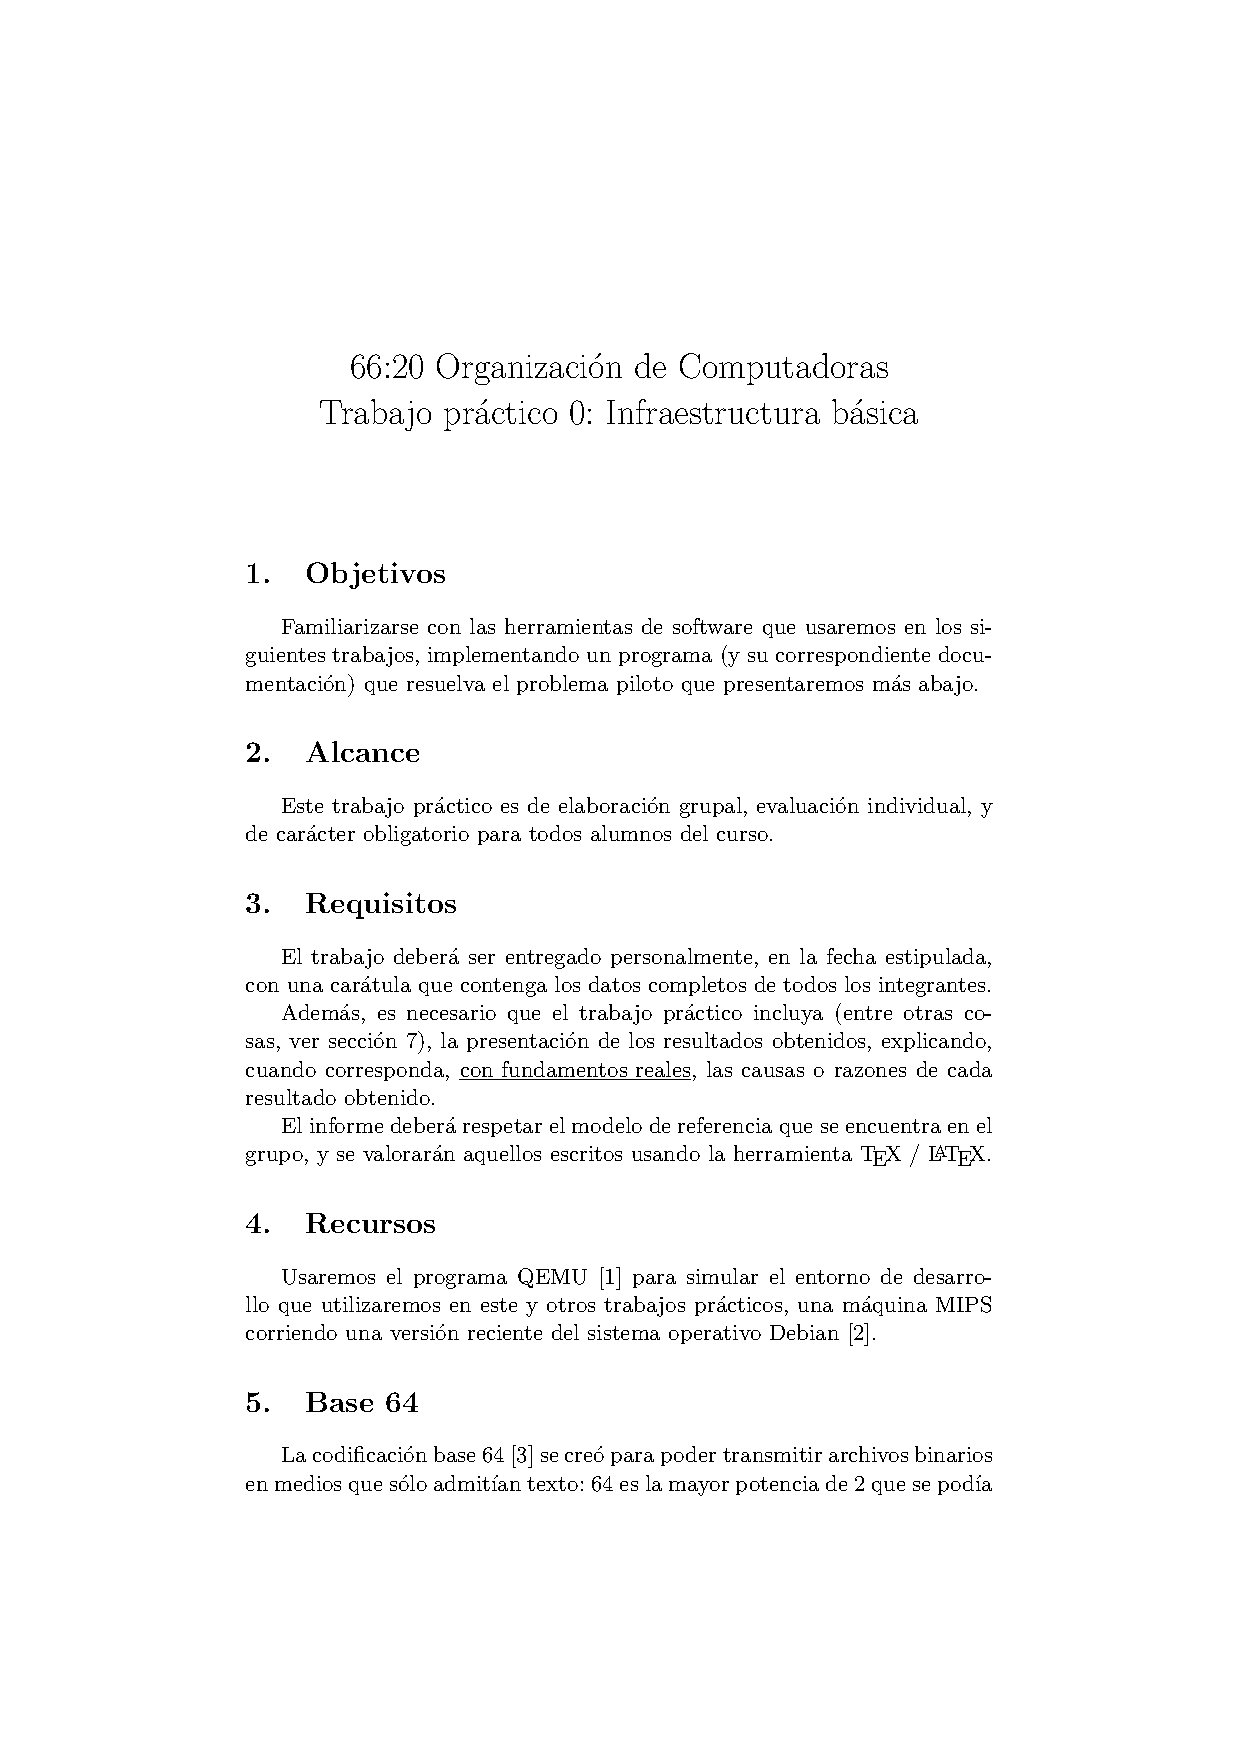
\includepdf[pages=1, scale=0.8, frame]{tp0-q2-2020.pdf}
\frame{
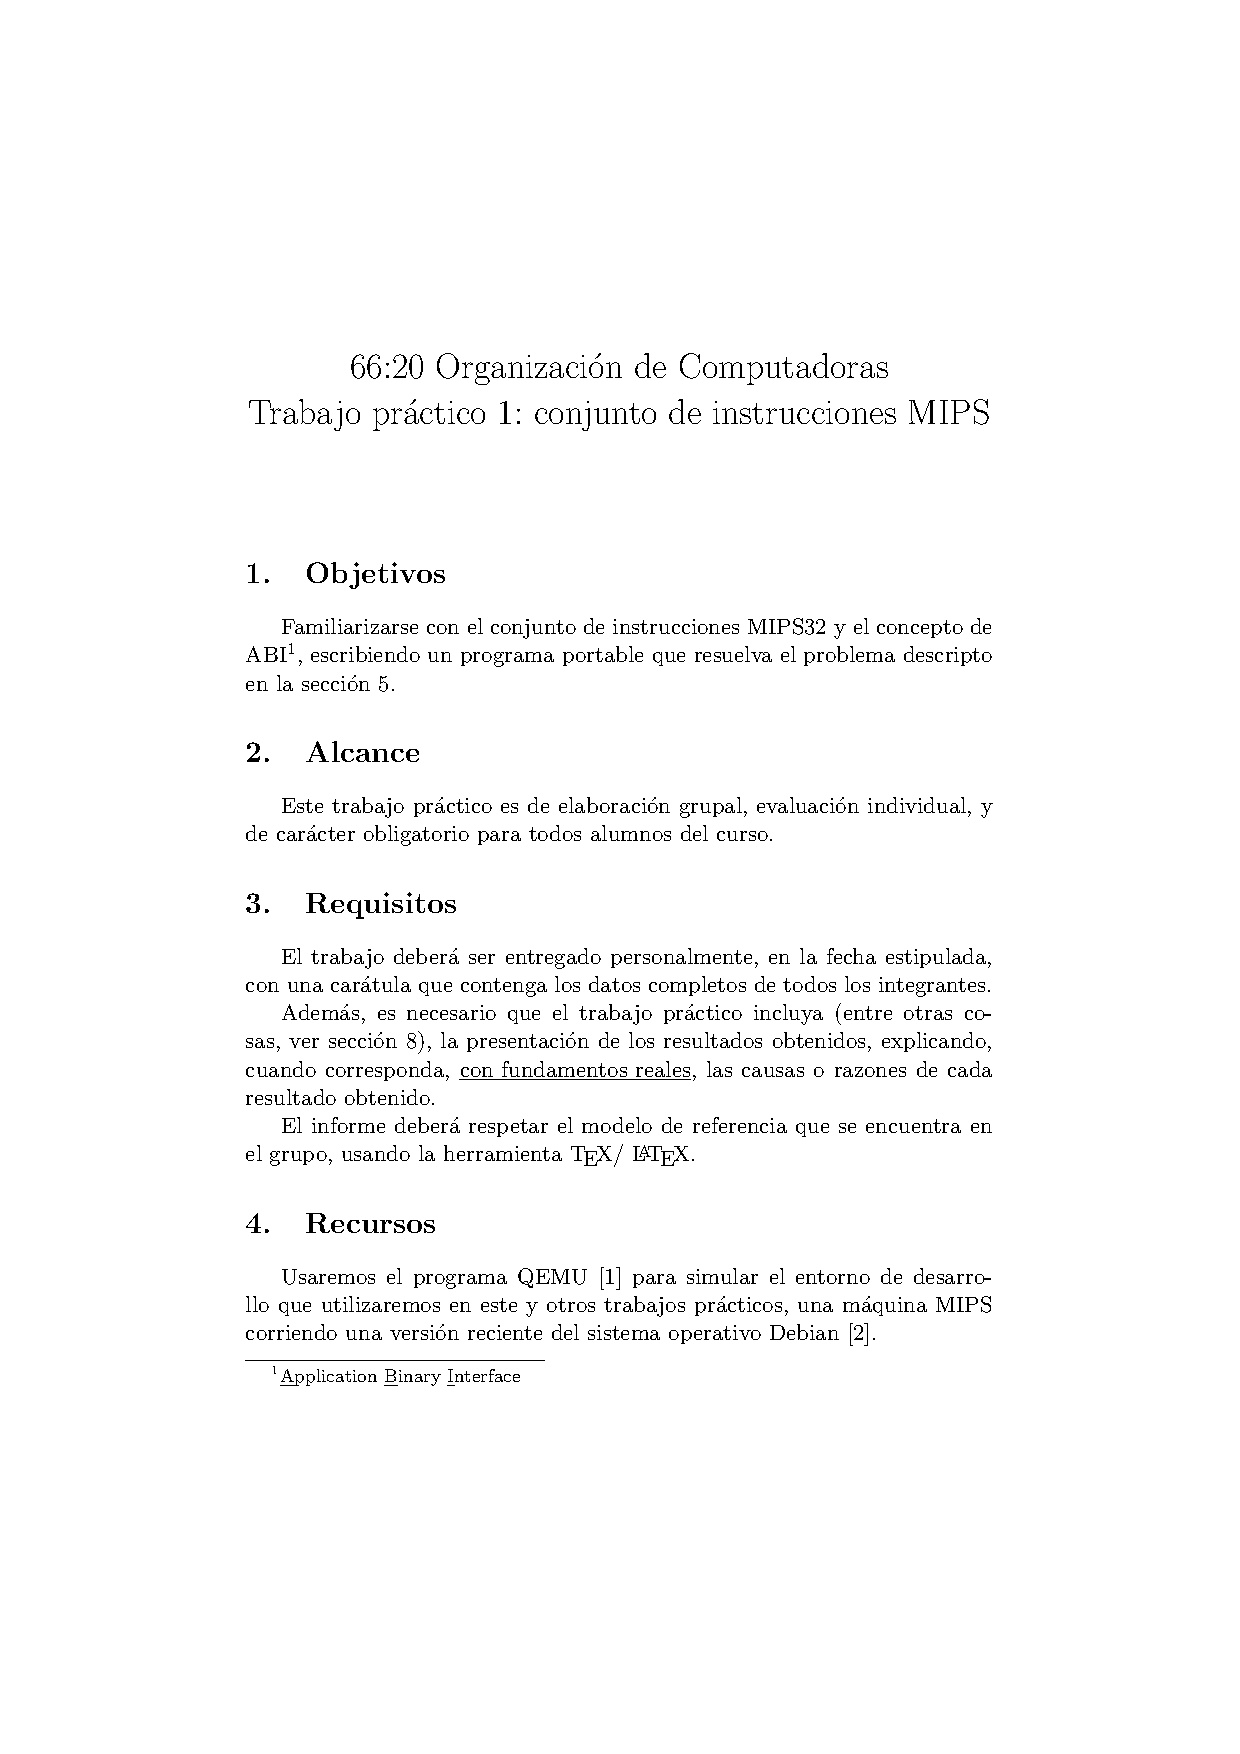
\includegraphics[height=0.93\textheight, frame]{tp1-q2-2020.pdf}
}
\includepdf[pages=2-, scale=0.8, frame]{tp1-q2-2020.pdf}
\newpage
\section{Código auxiliar}

\subsubsection{euclides algorithm.c}
\begin{lstlisting}[style=customC]

#include "euclides_algorithm.h"

unsigned int mcd_euclides(unsigned int a, unsigned int b) {
	unsigned int r = 0;
	
	if (b == 0) {
		return a;
	}
	r = (a % b);
	return mcd_euclides(b, r);
}

unsigned int mcm_euclides(unsigned int a, unsigned int b) {
	unsigned int mcd = mcd_euclides(a, b);
	unsigned int a_x_b = (a * b);
	return (a_x_b / mcd);
}

\end{lstlisting}

\newpage
\begin{thebibliography}{9}

\bibitem{euclidean_algorithm}
\cprotect\textit{Artículo de Wikipedia [en] sobre el Algoritmo de Euclides }. 
\href {https://en.wikipedia.org/wiki/Euclidean_algorithm}{
https://en.wikipedia.org/wiki/Euclidean_algorithm
}

\bibitem{gcc_parameters}
\cprotect\textit{Parámetros de \verb|gcc|}. 
\href {https://gcc.gnu.org/onlinedocs/gcc/Option-Summary.html}{
https://gcc.gnu.org/onlinedocs/gcc/Option-Summary.html
}

\bibitem{makefile}
\cprotect\textit{Herramienta \verb|make|}. 
\href {https://www.gnu.org/software/make/manual/make.html}{
https://www.gnu.org/software/make/manual/make.html
}



\end{thebibliography}

\end{document}